\documentclass[11pt,letter]{article}
%-------------------------
\usepackage{amsmath,amssymb}

\usepackage{amsthm}
\usepackage{mathrsfs}
\usepackage{bm}
\usepackage{ascmac} 
\usepackage{amsmath}
\usepackage{natbib} %
\usepackage{fancybox}
\usepackage{float}
\usepackage{booktabs} 
\usepackage{bm,xstring}
\usepackage{tabularx}
\usepackage{graphicx}
%\usepackage{mediabb}
\usepackage{lipsum}
\usepackage {pdfpages}
\usepackage{booktabs}
\usepackage{array}
\usepackage{paralist}
\usepackage{verbatim}
\usepackage{subfig} 
\usepackage{ascmac}
\usepackage{amsthm}
\usepackage{multirow}
\usepackage{amsmath}
\usepackage{natbib}
\usepackage{longtable}
\usepackage{hhline}
\usepackage{tabularx}
\usepackage{booktabs}
%\usepackage[T1]{fontenc}
\usepackage{textcomp}
\usepackage{here}
\usepackage{setspace}
\usepackage{color}
\usepackage{url}
\usepackage{xcolor}
%\usepackage{filecontents}
\usepackage{setspace}
\usepackage{fancyhdr}
\usepackage{titling}
\usepackage{titlesec}
\usepackage{sectsty}
\usepackage{listings}
\usepackage[many]{tcolorbox}
\usepackage[framemethod=TikZ]{mdframed}
\usepackage[dvipdfmx]{}
%\usepackage[dvipdfmx]{color}
\usepackage{epstopdf}
%\usepackage[dvipdfmx]{color}

\usepackage{bbm}
\usepackage{pdflscape}
\newcommand{\vect}[1]{\boldsymbol{\mathbf{#1}}}

%%%%%%%%%%%%%%%%%%%%%%%%%%%%%%
%Theorem
\newcounter{theo}[section] \setcounter{theo}{0}
\renewcommand{\thetheo}{\arabic{theo}}
\newenvironment{theo}[2][]{%
\refstepcounter{theo}%
\ifstrempty{#1}%
{\mdfsetup{%
frametitle={%
\tikz[baseline=(current bounding box.east),outer sep=0pt]
\node[anchor=east,rectangle,fill=gray!20]
{\strut Theorem~\thetheo};}}
}%
{\mdfsetup{%
frametitle={%
\tikz[baseline=(current bounding box.east),outer sep=0pt]
\node[anchor=east,rectangle,fill=gray!20]
{\strut Theorem~\thetheo:~#1};}}%
}%
\mdfsetup{innertopmargin=10pt,linecolor=gray!20,%
linewidth=2pt,topline=true,%
frametitleaboveskip=\dimexpr-\ht\strutbox\relax
}
\begin{mdframed}[]\relax%
\label{#2}}{\end{mdframed}}
%%%%%%%%%%%%%%%%%%%%%%%%%%%%%%
%Lemma
\newcounter{lem}[section] \setcounter{lem}{0}
\renewcommand{\thelem}{\arabic{section}.\arabic{lem}}
\newenvironment{lem}[2][]{%
\refstepcounter{lem}%
\ifstrempty{#1}%
{\mdfsetup{%
frametitle={%
\tikz[baseline=(current bounding box.east),outer sep=0pt]
\node[anchor=east,rectangle,fill=gray!50]
{\strut Lemma~\thelem};}}
}%
{\mdfsetup{%
frametitle={%
\tikz[baseline=(current bounding box.east),outer sep=0pt]
\node[anchor=east,rectangle,fill=gray!50]
{\strut Lemma~\thelem:~#1};}}%
}%
\mdfsetup{innertopmargin=10pt,linecolor=gray!50,%
linewidth=2pt,topline=true,%
frametitleaboveskip=\dimexpr-\ht\strutbox\relax
}
\begin{mdframed}[]\relax%
\label{#2}}{\end{mdframed}}
%%%%%%%%%%%%%%%%%%%%%%%%%%%%%%
%Assumption
\newcounter{asm}[section] \setcounter{asm}{0}
\renewcommand{\theasm}{\arabic{section}.\arabic{asm}}
\newenvironment{asm}[2][]{%
\refstepcounter{asm}%
\ifstrempty{#1}%
{\mdfsetup{%
frametitle={%
\tikz[baseline=(current bounding box.east),outer sep=0pt]
\node[anchor=east,rectangle,fill=gray!50]
{\strut Assumption~\theasm};}}
}%
{\mdfsetup{%
frametitle={%
\tikz[baseline=(current bounding box.east),outer sep=0pt]
\node[anchor=east,rectangle,fill=gray!50]
{\strut Assumption~\thelem:~#1};}}%
}%
\mdfsetup{innertopmargin=10pt,linecolor=gray!50,%
linewidth=2pt,topline=true,%
frametitleaboveskip=\dimexpr-\ht\strutbox\relax
}
\begin{mdframed}[]\relax%
\label{#2}}{\end{mdframed}}
%%%%%%%%%%%%%%%%%%%%%%%%%%%%%%
%Definition
\newcounter{defn}[section] \setcounter{defn}{0}
\renewcommand{\thedefn}{\arabic{section}.\arabic{defn}}
%\renewcommand{\thedefn}{\arabic{defn}}
\newenvironment{defn}[2][]{%
\refstepcounter{defn}%
\ifstrempty{#1}%
{\mdfsetup{%
frametitle={%
\tikz[baseline=(current bounding box.east),outer sep=0pt]
\node[anchor=east,rectangle,fill=gray!50]
{\strut Definition~\thedefn};}}
}%
{\mdfsetup{%
frametitle={%
\tikz[baseline=(current bounding box.east),outer sep=0pt]
\node[anchor=east,rectangle,fill=gray!50]
{\strut Definition~\thedefn:~#1};}}%
}%
\mdfsetup{innertopmargin=10pt,linecolor=gray!50,%
linewidth=2pt,topline=true,%
frametitleaboveskip=\dimexpr-\ht\strutbox\relax
}
\begin{mdframed}[]\relax%
\label{#2}}{\end{mdframed}}

%%%%%%%%%%%%%%%%%%%%%%%%%%%%%%
%Proof
\newcounter{prf}[section]\setcounter{prf}{0}
\renewcommand{\theprf}{\arabic{section}.\arabic{prf}}
\newenvironment{prf}[2][]{%
\refstepcounter{prf}%
\ifstrempty{#1}%
{\mdfsetup{%
frametitle={%
\tikz[baseline=(current bounding box.east),outer sep=0pt]
\node[anchor=east,rectangle,fill=gray!50]
{\strut Proof~\theprf};}}
}%
{\mdfsetup{%
frametitle={%
\tikz[baseline=(current bounding box.east),outer sep=0pt]
\node[anchor=east,rectangle,fill=gray!50]
{\strut Proof~\theprf:~#1};}}%
}%
\mdfsetup{innertopmargin=10pt,linecolor=gray!50,%
linewidth=2pt,topline=true,%
frametitleaboveskip=\dimexpr-\ht\strutbox\relax
}
\begin{mdframed}[]\relax%
\label{#2}}{\qed\end{mdframed}}
%%%%%%%%%%%%%%%%%%%%%%%%%%%%%%
%%%%%%%%%%%%%%%%%%%%%%%%%%%%%%
%Note
\newcounter{notes}[section] \setcounter{notes}{0}
\renewcommand{\thenotes}{\arabic{notes}}
\newenvironment{notes}[2][]{%
\refstepcounter{notes}%
\ifstrempty{#1}%
{\mdfsetup{%
frametitle={%
\tikz[baseline=(current bounding box.east),outer sep=0pt]
\node[anchor=east,rectangle,fill=gray!50]
{\strut Note~\thenotes};}}
}%
{\mdfsetup{%
frametitle={%
\tikz[baseline=(current bounding box.east),outer sep=0pt]
\node[anchor=east,rectangle,fill=gray!50]
{\strut Note~\thenotes:~#1};}}%
}%
\mdfsetup{innertopmargin=10pt,linecolor=gray!50,%
linewidth=2pt,topline=true,%
frametitleaboveskip=\dimexpr-\ht\strutbox\relax
}
\begin{mdframed}[]\relax%
\label{#2}}{\end{mdframed}}

\newtcolorbox{myboxi}[1][]{
  breakable,
  title=#1,
  colback=white,
  colbacktitle=white,
  coltitle=black,
  fonttitle=\bfseries,
  bottomrule=0pt,
  toprule=0pt,
  leftrule=3pt,
  rightrule=3pt,
  titlerule=0pt,
  arc=0pt,
  outer arc=0pt,
  colframe=black,
}


\usepackage{tgpagella}

\definecolor{mygreen}{RGB}{28,172,0} % color values Red, Green, Blue
\definecolor{mylilas}{RGB}{170,55,241}
\lstset{language=Matlab,%
    %basicstyle=\color{red},
    breaklines=true,%
    morekeywords={matlab2tikz},
    keywordstyle=\color{blue},%
    morekeywords=[2]{1}, keywordstyle=[2]{\color{black}},
    identifierstyle=\color{black},%
    stringstyle=\color{mylilas},
    commentstyle=\color{mygreen},%
    showstringspaces=false,%without this there will be a symbol in the places where there is a space
    numbers=left,%
    numberstyle={\tiny \color{black}},% size of the numbers
    numbersep=9pt, % this defines how far the numbers are from the text
    emph=[1]{for,end,break},emphstyle=[1]\color{red}, %some words to emphasise
    %emph=[2]{word1,word2}, emphstyle=[2]{style},    
}

%\usepackage[none]{hyphenat}
\usepackage{geometry}
\geometry{left=0.8in,right=0.8in, top=0.8in,bottom=0.8in}
\setlength\parindent{0pt}
%\renewcommand{\thesubsection}{(\alph{subsection})}
\usepackage{fancyhdr}
 

%\usepackage[shortlabels]{enumitem}
%                    \setlist[enumerate, 1]{1\textsuperscript{o}}


%--------------Shortcuts-----------
%Expectation
\newcommand{\Exp}[1]{\mathbb{E}\left[{#1}\right]}
\newcommand{\Var}[1]{\text{Var}\left[{#1}\right]}
\newcommand{\AsymVar}[1]{\text{AsymVar}\left[{#1}\right]}
\newcommand{\cov}[1]{\text{cov}\left[{#1}\right]}
\newcommand{\plim}[1]{\text{plim}\{{#1}\}}
\newcommand{\Ind}[1]{\mathbbm{1}\{{#1}\}}
\newcommand{\Prob}[1]{\text{Pr}\left({#1}\right)}
%hat
\newcommand{\h}[1]{\hat{#1}}
\newcommand{\thetahat}{\hat{\theta}}
\newcommand{\thetabar}{\overline{\theta}}
\newcommand{\gbar}{\overline{g}}
\newcommand{\psihat}{\hat{\psi}}

\newcommand{\vecty}{\vect{y}}

%upper and lower ber
\newcommand{\ob}[1]{\overline{#1}}
\newcommand{\ub}[1]{\underline{#1}}
\newcommand{\taubar}{\overline{\tau}}

%epsilon
\newcommand{\epsi}{\varepsilon}
\def\checkmark{\tikz\fill[scale=0.4](0,.35) -- (.25,0) -- (1,.7) -- (.25,.15) -- cycle;} 

\newcommand{\nonum}{\nonumber}

%ln()
\newcommand{\lnp}[1]{\ln\left({#1}\right)}

% parenthesis
\newcommand{\prn}[1]{\left({#1}\right)}
\newcommand{\mprn}[1]{\{{#1}\}}
\newcommand{\lmprn}[1]{\big\{{#1}\big\}}
\newcommand{\Lmprn}[1]{\Big\{{#1}\Big\}}
\newcommand{\llmprn}[1]{\biggl\{{#1}\biggr\}}
\newcommand{\LLmprn}[1]{\Biggl\{{#1}\Biggr\}}
\newcommand{\lprn}[1]{\left[{#1}\right]}

% cfrac
\newcommand{\cf}[2]{\cfrac{#1}{#2}}

% convergence in probability
\newcommand{\conp}{\xrightarrow{p}}
\newcommand{\cond}{\xrightarrow{d}}
\newcommand{\as}{\xrightarrow{a.s.}}

% Norm
\newcommand{\norm}[1]{\left\lVert{#1}\right\rVert}
\newcommand{\abs}[1]{\left\lvert{#1}\right\rvert}

\newcommand{\rootn}{\sqrt{n}}

\newcommand{\note}[1]{\ \ \ \ \text{#1}}

\newcommand{\ave}[1]{\frac{1}{#1}\sum_{i=1}^{#1}}

\newcommand{\half}{\cfrac{1}{2}}
\newcommand{\pihat}{\hat{\pi}}

\newcommand{\mbf}[1]{\mathbf{#1}}

\DeclareMathOperator*{\argmax}{argmax} 
\DeclareMathOperator*{\argmin}{argmin} 
\DeclareMathOperator*{\arginf}{arginf} 

\newcommand{\pmat}[1]{\begin{pmatrix} #1 \end{pmatrix}}%
\newcommand{\bmat}[1]{\begin{bmatrix} #1 \end{bmatrix}}%



\allowdisplaybreaks
\setstretch{1}

\newtheorem{definition}{Definition}

\newtheorem{lemma}{Lemma}
\newtheorem{assumption}{Assumption}
\newtheorem{theorem}{Theorem}

\newcommand{\code}[1]{\texttt{#1}}

\bibliographystyle{aer} 

%----------------------------------------------------------------------------------------
%	TITLE SECTION
%----------------------------------------------------------------------------------------

\newcommand{\horrule}[1]{\rule{\linewidth}{#1}} % Create horizontal rule command with 1 argument of height

\title{	
\normalfont \normalsize 
\textsc{Penn State, Spring 2019, ECON512 Empirical Method} \\ [25pt] % Your university, school and/or department name(s)
\horrule{0.5pt} \\[0.4cm] % Thin top horizontal rule
\huge Homework 6 \\ % The assignment title
\horrule{2pt} \\[0.5cm] % Thick bottom horizontal rule
}

\author{Kensuke Suzuki} % Your name

\date{\normalsize\today} % Today's date or a custom date

\pagestyle{fancy}
\fancyhf{}
\chead{ECON512 Homework 6 -- Kensuke Suzuki}
\lhead{}
\rfoot{\thepage}

\begin{document}

\maketitle % Print the title


%%%%%%%%%%%%%%%%%%%%%%
\section*{Problem 1: Dynamic optimization problem}

Firm's current period payoff is

\begin{align}
\pi(x_t, p_t) = p_t \cdot x_t - 0.2 \cdot x_t^{1.5} 
\end{align}

We want to make the stock of lumber as a state variable, so that $x=k-k'$.  Then equation (1) can be written as

\begin{align}
\pi(k_t,k_{t+1},p_t) = p \cdot (k_{t}-k_{t+1}) - 0.2 \cdot (k_{t}-k_{t+1})^{1.5}
\end{align}

Then we can formulate the firm's problem such that it chooses $k'$ (next period stock) given the state variables $(k,p)$. The Bellman's equation is

\begin{align}
V(k,p) = \max_{k'}  p \cdot (k-k') - 0.2 \cdot (k-k')^{1.5} + \delta \mathbb{E}_{p'}\lprn{V(k',p')|p}
\end{align}

given initial stock of lumber (between 0 and 100) and transition probability of $p$ which is defined by the AR(1) process ($p'= p_0 + \rho\cdot p + u$). In the Bellman's equation presented in equation (2), expectation is taken over next period price $p'$ given today's price $p$.


%%%%%%%%%%%%%%%%%%%%%%
\section*{Problem 2: Tauchen}

I use \code{tauchen.m} to generate grid that approximate process for $p_t$ for given AR(1) parameters. Variable \code{grid} stores the grid points for $p_t$ and \code{prob} stores the transition probabilities.

\newpage
%%%%%%%%%%%%%%%%%%%%%%
\section*{Problem 3: Value function iteration (VIF)}

The basic structure of the VIF algorithm is analogous to the one provided in the lecture. Note that:
\begin{itemize}
\item \code{harvest} stores the harvest for given current stock (in column) and next period stock (in raw)
\item I penalize the negative revenue by replacing with $-1e6.0$
\item In order to avoid imaginary number, before calculating the current payoff (profit), I replace the negative harvest with 0.
\end{itemize}
 
I plot the value of the firm depending on its initial stock (x-axis) and the current price of lumber. 

\begin{figure}[h]
\begin{center}
\caption{Problem 3}
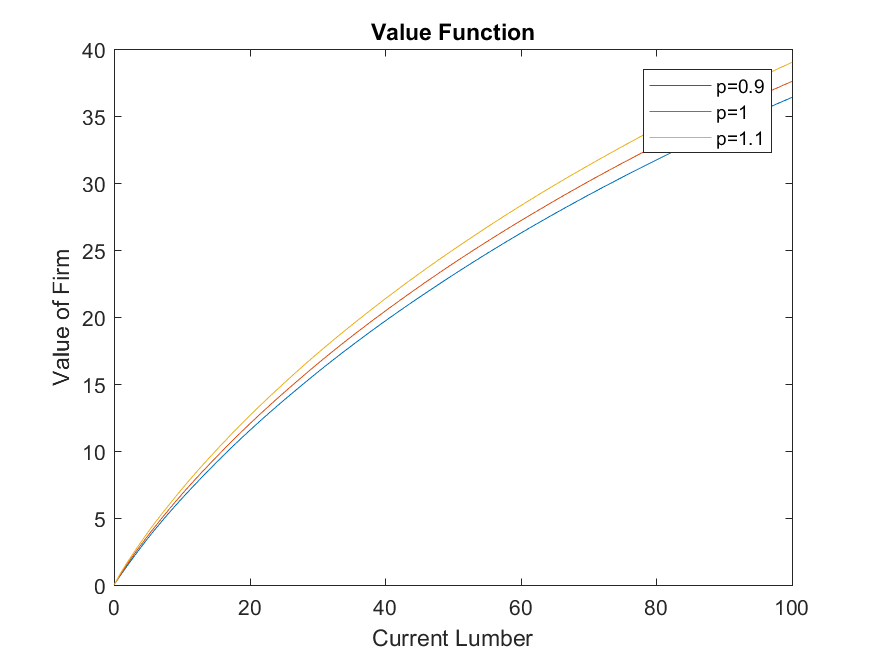
\includegraphics[width=0.7\textwidth]{prob3.png}
\end{center}
\end{figure}

\newpage
%%%%%%%%%%%%%%%%%%%%%%
\section*{Problem 4: Next period stock as a function of price}

I plot next period optimal stock as a function of today's price for different amount of lumber left in stock.

\begin{figure}[h]
\begin{center}
\caption{Problem 4}
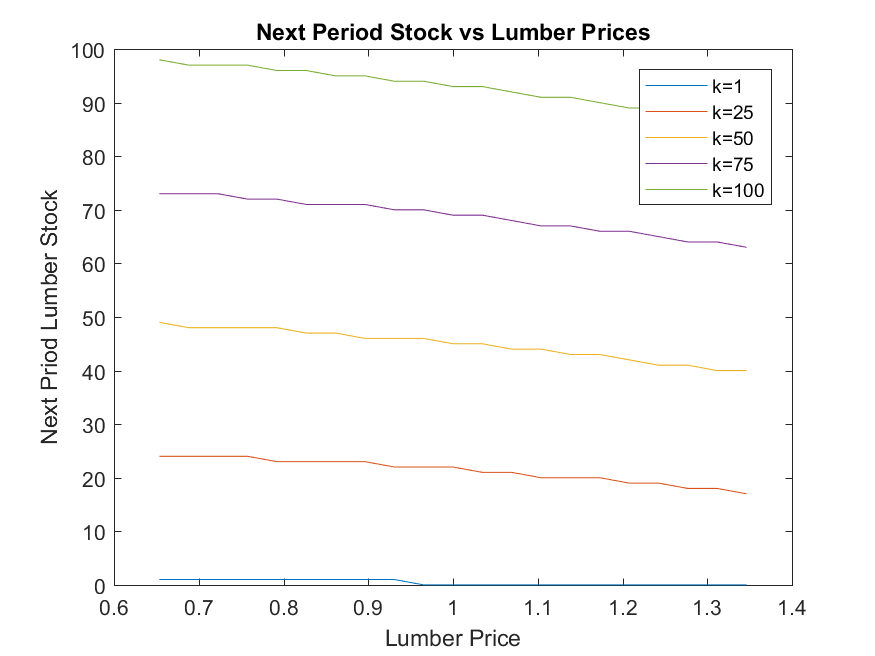
\includegraphics[width=0.7\textwidth]{prob4.png}
\end{center}
\end{figure}

\newpage
%%%%%%%%%%%%%%%%%%%%%%
\section*{Problem 5: Expected path of lumber stock}


Using the code provided in the class, I first construct the transition probability matrix of the state ($k,p$) by combining the transition matrix of price and the decision rule matrix. Given the initial state ($k=100,p=1$), we can construct the initial probability distribution matrix, which has a mass (1) on $k=100$ and $p=1$. Then, using the transition matrix of the state, we can generate the next period probability distribution over state ($k,p$). By integrating (summing) over all possible price values, we can obtain the expected lumber stock. We can also obtain the lower and upper bound of confidence interval by obtaining 5\% and 95\%tile of the marginal distribution of $k$ in each period. We repeat this for 20 periods. In the figure below, $t=1$ is the starting point, so we compute the expected path and the confidence interval from $t=2$ to $t=21$.

%
%I compute the expected path in the following way.
%
%\begin{enumerate}
%\item Simulate the path of price for 20 period ($p_t$ for $t\in[1,20]$), given $p_0=1$, as follows.
%\begin{itemize}
%\item Using the transition probability matrix, compute the \textit{cumulative probability} for given current period price ($p_{t}$). \code{cdf} is the vector where $i$th element stores $cdf_i = \sum_{j=1}^i = \pi(p_j | p_{t})$.
%\item Draw a uniform random variable $r\in[0,1]$ using \code{rand} and find the smallest index $i$ such that $cdf_i>r$. Then set the next priod price as $p_{t+1}=p_i$. 
%\end{itemize}
%\item Using the path of price obtained in Step 1, we can compute the path of lumber stock. Next period lumber stock is determined by the decision rule which is obtained in Problem 3 above. Denote the path of lumber stock obtained in this step by $k_t^s$ for $t=1,2,...,20$. $s$ is the index of the simulation, which is explained below.
%\item Repeat the Step 1--2 for $S=1000$ times, $s=1,2,...,S$. Expected lumber stock is computed as the sample average of $k_t^s$: $\overline{k}_t = \frac{1}{S}\sum_{s=1}^{S} k_t^s$.
%
%Confidence interval is obtained by
%\begin{align*}
%\overline{k}_t - t_{0.05}(S-1)\frac{SD_t}{\sqrt{S}}<\Exp{k_t}<\overline{k}_t + t_{0.05}(S-1)\frac{SD_t}{\sqrt{S}}
%\end{align*}
%where $t_{0.05}(S-1)$ and $t_{0.95}(S-1)$, respectively, are 5\%tile and 95\%tile of $t$-distribution with degree of freedom $S-1$. $std_t$ is the standard deviation of $k_t^s$: $SD_t= \sqrt{\frac{1}{S-1}\sum_{s=1}^S\abs{k_t^s-\overline{k}_t}}$. 
%\end{enumerate}


\begin{figure}[h]
\begin{center}
\caption{Problem 5}
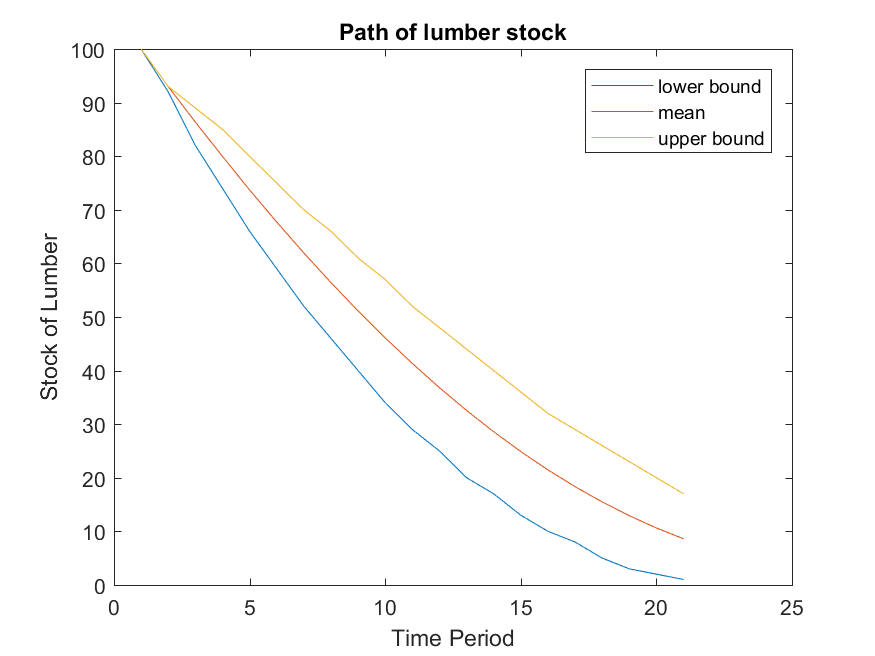
\includegraphics[width=0.7\textwidth]{prob5_2.png}
\end{center}
\end{figure}


\newpage

%%%%%%%%%%%%%%%%%%%%%%
\section*{Problem 6: Results with coarse grid}

\subsection*{Problem 6-2: Tauchen}
I now use 5 grid points and generate the grid and transition probability for $p_t$.

\subsection*{Problem 6-3: VIF}
\begin{figure}[h]
\begin{center}
\caption{Problem 6-3}
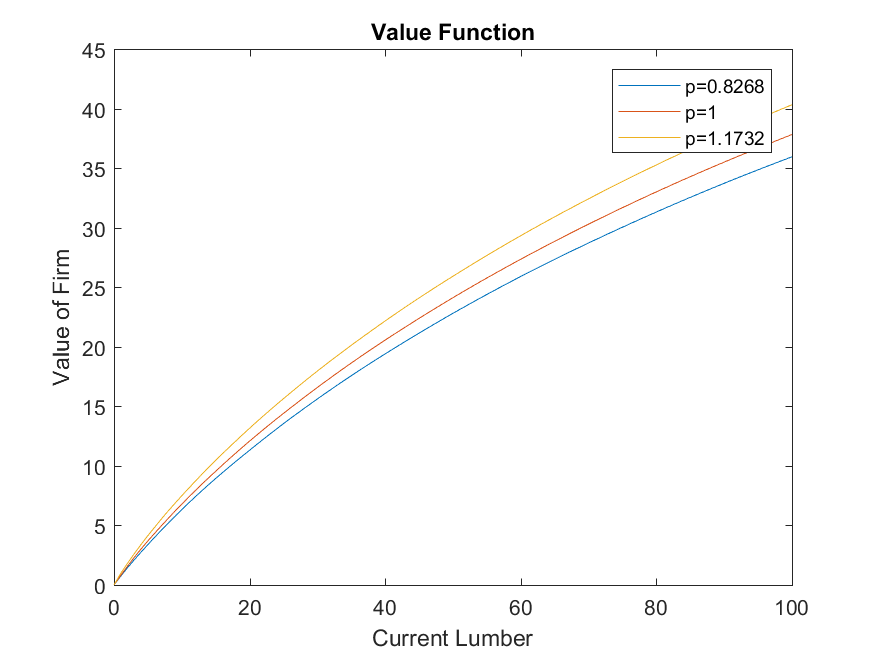
\includegraphics[width=0.7\textwidth]{prob6_1.png}
\end{center}
\end{figure}

\newpage
\subsection*{Problem 6-4: Next period stock as a function of price}
\begin{figure}[h]
\begin{center}
\caption{Problem 6-4}
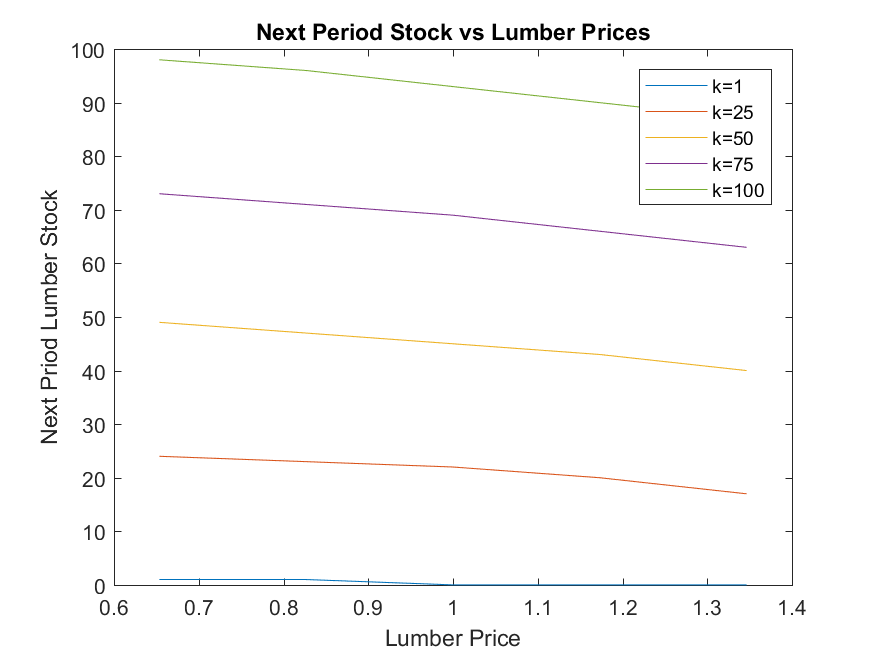
\includegraphics[width=0.7\textwidth]{prob6_2.png}
\end{center}
\end{figure}

\newpage
\subsection*{Problem 6-5: Expected stock}
\begin{figure}[h]
\begin{center}
\caption{Problem 6-5}
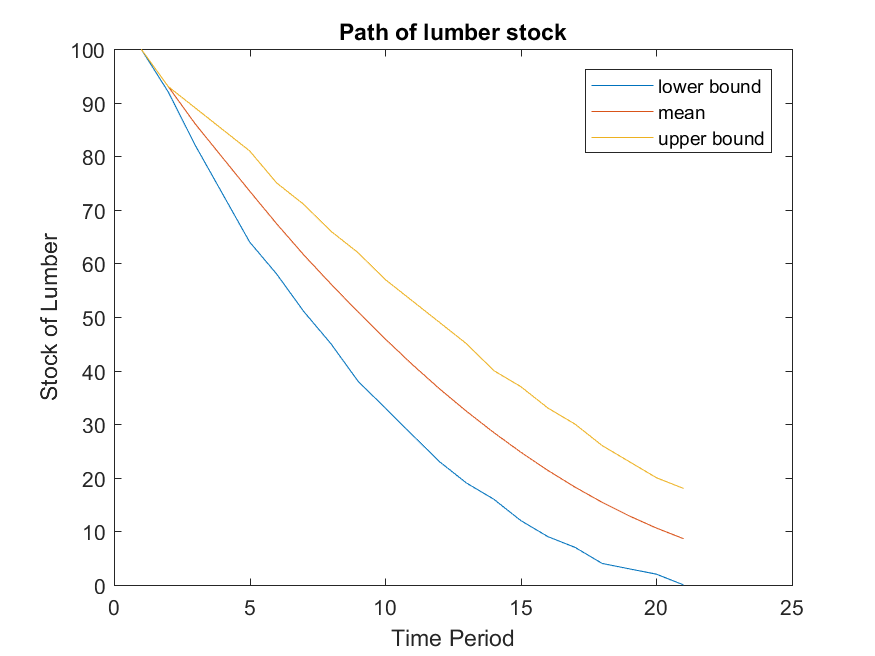
\includegraphics[width=0.7\textwidth]{prob6_3_2.png}
\end{center}
\end{figure}

\newpage
%%%%%%%%%%%%%%%%%%%%%%
\section*{Matlab Main Code}
\lstinputlisting{HW6.m}


\end{document}  



  